\def \equationFirst {\dfrac{dx}{dt} = (\alpha - \beta \cdot y) \cdot x} 
\def \equationSecond {\dfrac{dy}{dt} = (\delta \cdot x - \gamma) \cdot y} 

\def \system {$
	\begin{dcases*} 
		\equationFirst \\
		\equationSecond
	\end{dcases*}
$}

\def \conditions {
	$ x(0) = y(0) = 1 $
	 
	$ \alpha = \gamma = 0.76  $
	
	$ \beta = \delta = 0.62  $
}

\definecolor{bgcolor}{RGB}{255,254,235}
\definecolor{base0}{RGB}{131,148,150}
\definecolor{base01}{RGB}{88,110,117}
\definecolor{base2}{RGB}{238,232,213}
\definecolor{sgreen}{RGB}{133,153,0}
\definecolor{sblue}{RGB}{38,138,210}
\definecolor{scyan}{RGB}{42,161,151}
\definecolor{smagenta}{RGB}{211,54,130}

\newcommand\digitstyle{\color{smagenta}}
\newcommand\symbolstyle{\color{base01}}

\makeatletter
\newcommand{\ProcessDigit}[1]
{%
	\ifnum\lst@mode=\lst@Pmode\relax%
	{\digitstyle #1}%
	\else
	#1%
	\fi
}
\makeatother


\lstdefinestyle{solarizedcpp} {
	language=C,
	breaklines=true,
	frame=single,
	tabsize=2,
	breakatwhitespace=true,
	captionpos=b,
	backgroundcolor=\color{bgcolor},
	basicstyle=\footnotesize\ttfamily,
	keywordstyle=\bfseries\color{sgreen},
	showstringspaces=false,
	identifierstyle=\color{sblue},
	extendedchars=true,
	literate=
	{*0}{{{\ProcessDigit{0}}}}1
	{*1}{{{\ProcessDigit{1}}}}1
	{*2}{{{\ProcessDigit{2}}}}1
	{*3}{{{\ProcessDigit{3}}}}1
	{*4}{{{\ProcessDigit{4}}}}1
	{*5}{{{\ProcessDigit{5}}}}1
	{*6}{{{\ProcessDigit{6}}}}1
	{*7}{{{\ProcessDigit{7}}}}1
	{*8}{{{\ProcessDigit{8}}}}1
	{*9}{{{\ProcessDigit{9}}}}1
	{*\}}{{\symbolstyle{\}}}}1
	{*\{}{{\symbolstyle{\{}}}1
	{*(}{{\symbolstyle{(}}}1
	{*)}{{\symbolstyle{)}}}1
	{*=}{{\symbolstyle{$=$}}}1
	{*;}{{\symbolstyle{$;$}}}1
	{*>}{{\symbolstyle{$>$}}}1
	{*<}{{\symbolstyle{$<$}}}1
	{**}{{\symbolstyle{*}}}1
	{*\%}{{\symbolstyle{$\%$}}}1,
}

\lstset{escapechar=@, style=solarizedcpp}


\newcommand {\solutionItemThird} {
	\textit{Код:}
		\lstinputlisting{code/main.c}
	
	\clearpage
	
	\textit{Графики:}
	\begin{figure}[h]
		\centering
		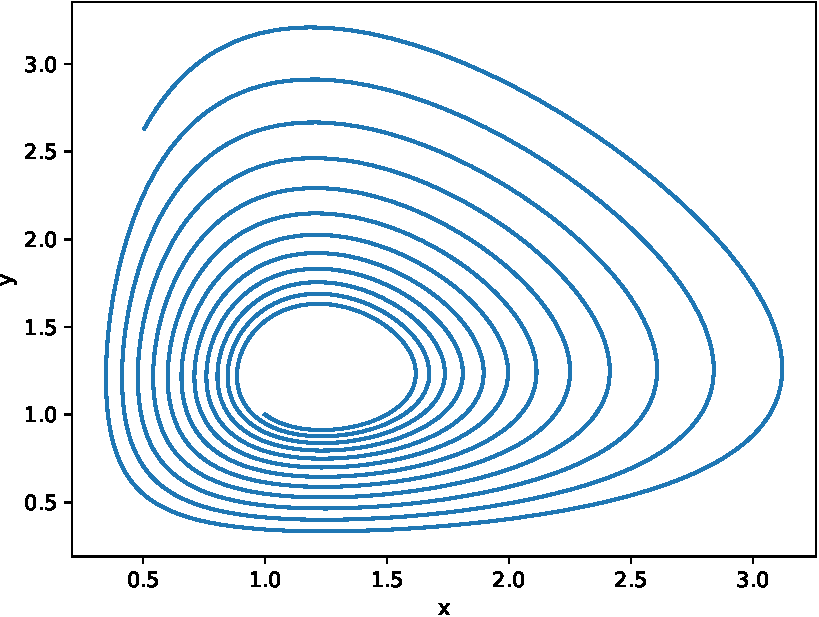
\includegraphics[scale=0.7]{img/dist/predator1.pdf}
	\end{figure}

	\begin{figure}[h]
		\centering
		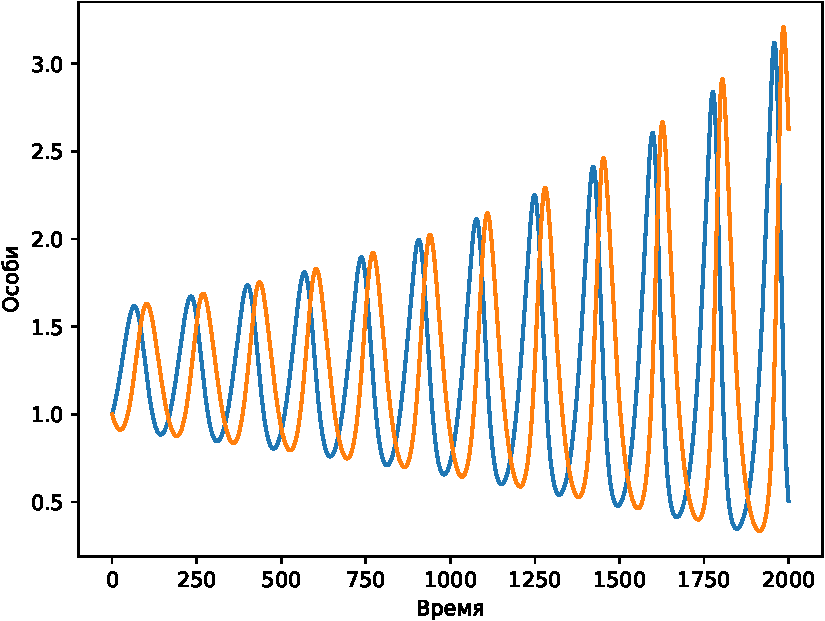
\includegraphics[scale=0.7]{img/dist/predator2.pdf}
	\end{figure}
}

\section{Задача 3.}
\subsection{Постановка задачи}
Для модели «Хищник-Жертва» описать поведение решений соответствующих
уравнений системы при заданных коэффициентах. Построить график решения.\\
Реализацию программы провести на языке «С».

\begin{enumerate}[label={}]
	\item \system
	\item \conditions
\end{enumerate}


\newpage

\subsection{Решение}
\solutionItemThird
